\graphicspath{{chapters/c4_azurin_sm/si/}}
%=====================METHODS AND FIGURES===========================
\section{Supporting info}
\begin{figure}[ht]
  \centering
  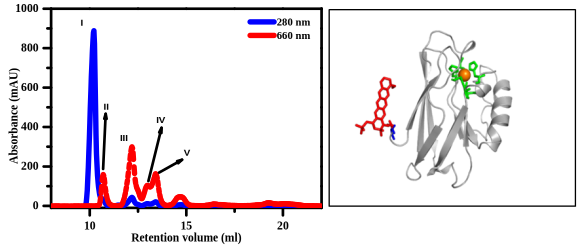
\includegraphics[width=0.8\textwidth]{peak_separation}
  \makeatletter
  \renewcommand{\fnum@figure}{\figurename~S\thefigure}
  \makeatother
  \caption{Peak separation: (a) Elution profile of a Cu-azurin sample after labeling and removal of free dye.
  The \SI{280}{\nm} absorption that shows the presence of protein is shown in blue and the \SI{660}{\nm} absorption that refers to the presence of dye is shown in red.
  The protein structure with the dye at Lys corresponding to peak-III is shown at the right. 
  }
  \label{SIfig: peak_sep}
\end{figure}
%==================BULK Switching=========================
\paragraph*{Fluorescence switching in bulk.} Fluorescence measurements in bulk of different peaks of azurin-ATTO655 sample (Figure S\ref{SIfig: peak_sep}) related to different positions of the dye on the protein surface were carried out to determine the FRET switching ratio.
The measurements were done in Cary Eclipse Spectrometer (Varian Inc. Agilent Technology, USA).
A \SI{50}{\nM} sample was excited with \SI{665}{\nm} laser and the intensity was monitored above \SI{675}{\nm}.
Sodium ascorbate (reductant) and pottasium ferricyanide (oxidant) were added alternatively.
Among all the labeled positions, peak-III showed maximum switching ratio and its intensity change can be seen in Figure S\ref{SIfig: switching}.
Similarly Zn Azurin-ATTO655 showed little or no change in intensity.

\begin{figure}[ht]
  \centering
  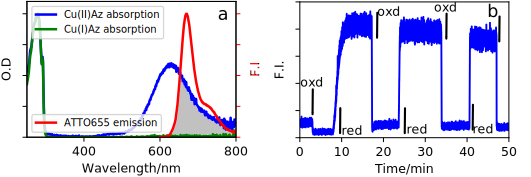
\includegraphics[width=\textwidth]{spectral_overlap_switching}
  \makeatletter
  \renewcommand{\fnum@figure}{\figurename~S\thefigure}
  \makeatother
  \caption{ \textbf{Spectral overlap and Bulk switching:} (a) Absorption spectrum of Cu(II)azurin (green), Cu(I)azurin (blue).
  The emission spectrum of ATTO655 (red) has a good overlap with the absorption of Cu(II)azurin to show high FRET. 
  (b) Fluorescence intensity of \SI{50}{\nM} CuAzurin-ATTO655 shows high intensity in the presence of reductant and low 
  intensity with oxidant.
  The switching ratio is \SI{90}{\percent} which satisfies the requirement for single-molecule FRET.
  }
  \label{SIfig: switching}
\end{figure}
%==================time trace Zn and Cu azurin=================
\begin{figure}[ht]
  \centering
  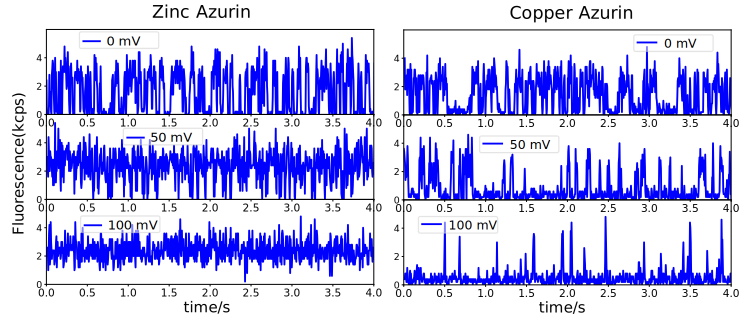
\includegraphics[width=\textwidth,keepaspectratio]{SI_timetrace_Zn_Cu}
  \makeatletter
  \renewcommand{\fnum@figure}{\figurename~S\thefigure}
  \makeatother
  \caption{Time traces of Zn-azurin (left) and of Cu-azurin(right) labeled with ATTO655 at different potentials. 
  Above \SI{40}{\mV}, Cu-Azurin shows switching in the intensity due to changes in the oxidation state of the copper metal center and below \SI{40}{\mV}, triplet blinking contributes to the switching as can be seen in the redox inactive Zn-Azurin.
  To keep the analysis simple, time traces above \SI{40}{\mV} were choosen for Cu-azurin.
  }
  \label{SIfig:tracecomparision}
\end{figure}
%===================lifetime and switching ration from time trace================
\begin{figure}
  \centering
  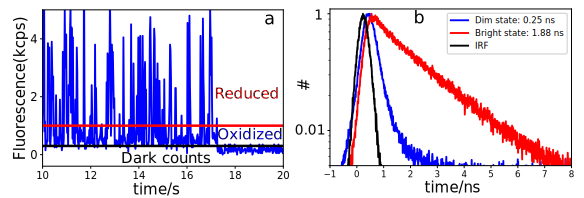
\includegraphics[width=\textwidth]{lifetime}
  \makeatletter
  \renewcommand{\fnum@figure}{\figurename~S\thefigure}
  \makeatother
  \caption{\textbf{Single-molecule azurin switching and lifetime.} (a) Time trace of a single Cu azurin at \SI{50}{\mV} with a binning time of \SI{50}{\ms}.
  Notice the three different labels indicated in the figure.
  Bright (Cu(I)) state as above the red line, oxidized state is between red and black line and Dark counts are below the black line.
  The fact that the molecule does not go to the dark count label before being bleached shows that the transitions are due to copper oxidation switching rather than triplet blinking of the dye.
  Once the fluorophore is bleached, transitions were no longer observable.
  (b) The lifetime histogram corresponding to bright state (red), oxidized state (blue) and instrument response function (black).
  The lifetime of the oxidized state is much shorter than that of the reduced state due to FRET quenching.}
  \label{SIfig: lifetime}
\end{figure}
%=====================FCS comparision=========================
\begin{figure}[ht]
  \centering
  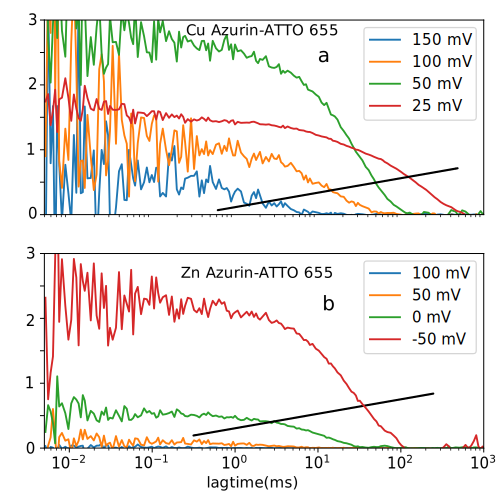
\includegraphics[width=\textwidth]{fcs_comparision}
  \makeatletter
  \renewcommand{\fnum@figure}{\figurename~S\thefigure}
  \makeatother
  \caption{Autocorrelation of time traces of Cu azurin-ATTO655 (a) and Zn azurin-ATTO655 (b) at different potential. 
  At lower potential, Cu-azurin-ATTO655 has longer correlation time (on time), which shows that the molecule spends more time on the Cu(I) state.
  But below \SI{50}{\mV} the dye (ATTO655) starts to show triplet blinking.
  As the potential is lowered the triplet blinking dominates.
  The Cu-azurin study is focused in the safe window of potentials more than \SI{40}{\mV} where triplet blinking is absent.}
  \label{SIfig:fcscomparision}
\end{figure}
\squeezeup
%===============================Slope: Nernst equation==================================
\begin{figure}[ht]
  \centering
  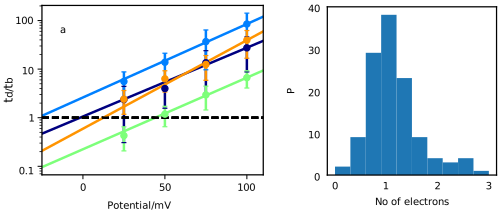
\includegraphics[width=0.8\textwidth]{SI_potential_slope}
  \makeatletter
  \renewcommand{\fnum@figure}{\figurename~S\thefigure}
  \makeatother
  \caption{(a) Fitting of the ratio between bright and dark times with Nernst equation with slope as variable parameters for Cu-Azurin ATTO655. 
  (b) The corresponding histogram of slopes obtained from the fitting shown in the left.
  The distribution of slope is centered around \SI{59}{\mV} indicating that Cu-azurin switching  involves only one electron.}
  \label{SIfig:potential_slope}
\end{figure}
\squeezeup
%===================================Rate fit at all potential=============================
\begin{figure}[ht]
  \centering
  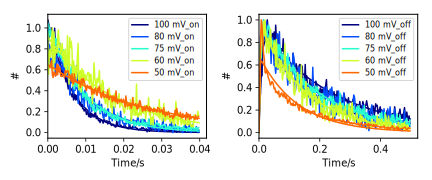
\includegraphics[width=\textwidth]{rate_fit_all_potential}
  \makeatletter
  \renewcommand{\fnum@figure}{\figurename~S\thefigure}
  \makeatother
  \caption{(a) Fitting of $bright-time$ distribution with mono-exponential at different potentials.
  (a) Fitting of $dark-times$ distribution with bi-exponential equation with rise time as shown in the main text at different potentials.
  The characteristic decay constants were plotted against potential (see main text).}
  \label{SIfig: rate_fit_all_potential}
\end{figure}

% =============== Dynamic heterogenity ==================
\clearpage
\paragraph*{Examples of dynamic heterogeneity in different molecules}
Different azurin molecules show different dynamic patterns of dynamic heterogeneity.
As the number of conformations azurin can possess is large, we could not obtain reliable histogram of the times the protein takes to convert from one conformation to another.
Figure S\ref{SIfig:dynamic_trace_steps}, S\ref{SIfig:dynamic_Point_20_75mV_S105}, S\ref{SIfig:dynamic_Point_21_75mV_S105} show three different azurin molecules with very different dynamics.
Correlation of bright and dark times of  different molecules are shown in Figure S\ref{SIfig:Dynamic_corr_many}.

\begin{figure}[ht]
  \centering
  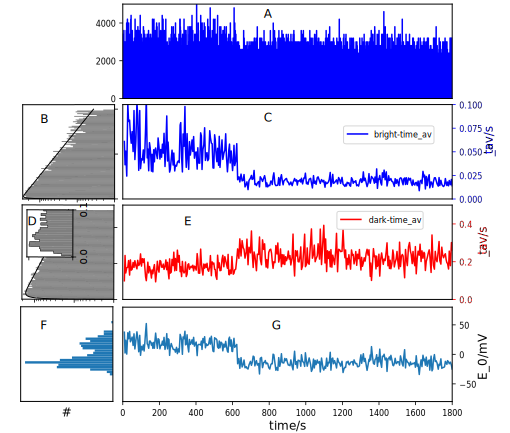
\includegraphics[width=\textwidth]{dynamic_trace_steps}
  \makeatletter
  \renewcommand{\fnum@figure}{\figurename~S\thefigure}
  \makeatother
  \caption{\textbf{Example 2: Dynamic heterogeneity of azurin-ATTO655}
  A long time trace (A) of Cu-azurin-ATTO655 at \SI{50}{\mV} with zoom-in (A, B) at different point of its time course.
  Variation of bright times (C) and dark times(E) of the same azurin with their histogram on the left.
  The times were averaged over every ten consecutive ones to get rid of noise and for easy visualization.
  The trace of midpoint potential(G) calculated from the bright- and dark-times and the the histogram(F) of midpoint potential is shown on its left.
  Along with variation at shorter time scales (tens of seconds), the molecule shows a major step like change.
  The distribution of midpoint potential shows two peaks with values at around \SI{20}{\mV} and \SI{-20}{\mV}.
  }
  \label{SIfig:dynamic_trace_steps}
\end{figure}

\begin{figure}[!ht]
  \centering
  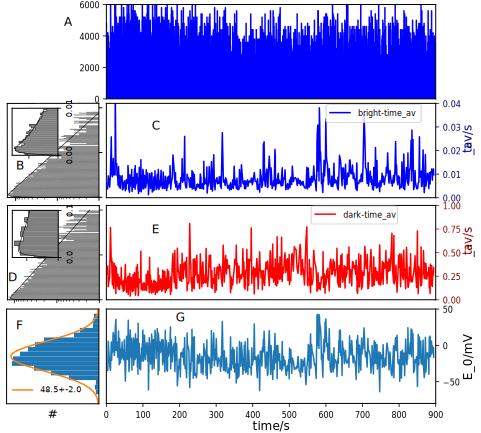
\includegraphics[width=\textwidth]{dynamic_Point_20_75mV_S105}
  \makeatletter
  \renewcommand{\fnum@figure}{\figurename~S\thefigure}
  \makeatother  
  \caption{\textbf{Example 3: Dynamic heterogeneity of azurin-ATTO655}
  A long time trace (A) of Cu-azurin-ATTO655 at \SI{50}{\mV} with zoom-in (A, B) at different point of its time course.
  Variation of bright times (C) and dark times(E) of the same azurin with their histogram on the left.
  The times were averaged over every ten consecutive ones to get rid of noise and for easy visualization.
  The trace of midpoint potential(G) calculated from the bright- and dark-times and the the histogram(F) of midpoint potential is shown on its left.
  }
  \label{SIfig:dynamic_Point_20_75mV_S105}
\end{figure}

\begin{figure}[ht]
  \centering
  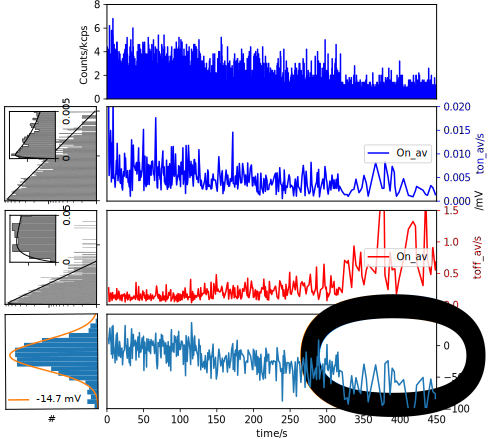
\includegraphics[width=\textwidth]{dynamic_Point_21_75mV_S105}
  \makeatletter
  \renewcommand{\fnum@figure}{\figurename~S\thefigure}
  \makeatother
  \caption{\textbf{Example 4: Dynamic heterogeneity of azurin-ATTO655}
  A long time trace (A) of Cu-azurin-ATTO655 at \SI{50}{\mV} with zoom-in (A, B) at different point of its time course.
  Variation of bright times (C) and dark times(E) of the same azurin with their histogram on the left.
  The times were averaged over every ten consecutive ones to get rid of noise and for easy visualization.
  The trace of midpoint potential(G) calculated from the bright- and dark-times and the the histogram(F) of midpoint potential is shown on its left.
  }
  \label{SIfig:dynamic_Point_21_75mV_S105}
\end{figure}

\begin{figure}[ht]
  \centering
  \includegraphics[width=0.8\textwidth]{Dynamic_corr_many}
  \makeatletter
  \renewcommand{\fnum@figure}{\figurename~S\thefigure}
  \makeatother
  \caption{\textbf{Dynamic correlations.}
  Correlation of bright times and dark times for different molecules.
  Notice the different characteristic decay time for different molecules which can vary from seconds to tens of seconds.
  The plot on the bottom right has flat correlation with no decay indicating absence of any heterogeneity with the observation times.  
  }
  \label{SIfig:Dynamic_corr_many}
\end{figure}

%===================================No of averaging points=================================
\begin{figure}[!ht]
  \centering
  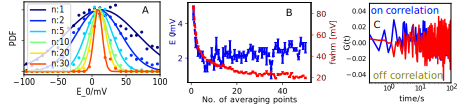
\includegraphics[width=\textwidth]{N_avgpoints_vs_fwhmwidth}
  \makeatletter
  \renewcommand{\fnum@figure}{\figurename~S\thefigure}
  \makeatother
  \caption{\textbf{No correlation dynamics.} Variation of midpoint potential and fwhm with the number of bright- and dark-times taken for averaging for the long trace shown in the main text (Figure-\ref{fig:long_azurin_trace}). At around $20~$ events, both $E_0$ and fwhm reaches plateau.
  The averaging of bright-time and dark-times for correlation and midpoint distribution were done every $20$ events.}
  \label{SIfig: N_avgpoints_vs_fwhmwidth}
\end{figure}

% %============on-off 2D histogram=============

% \begin{figure}[ht]
%   \centering
%   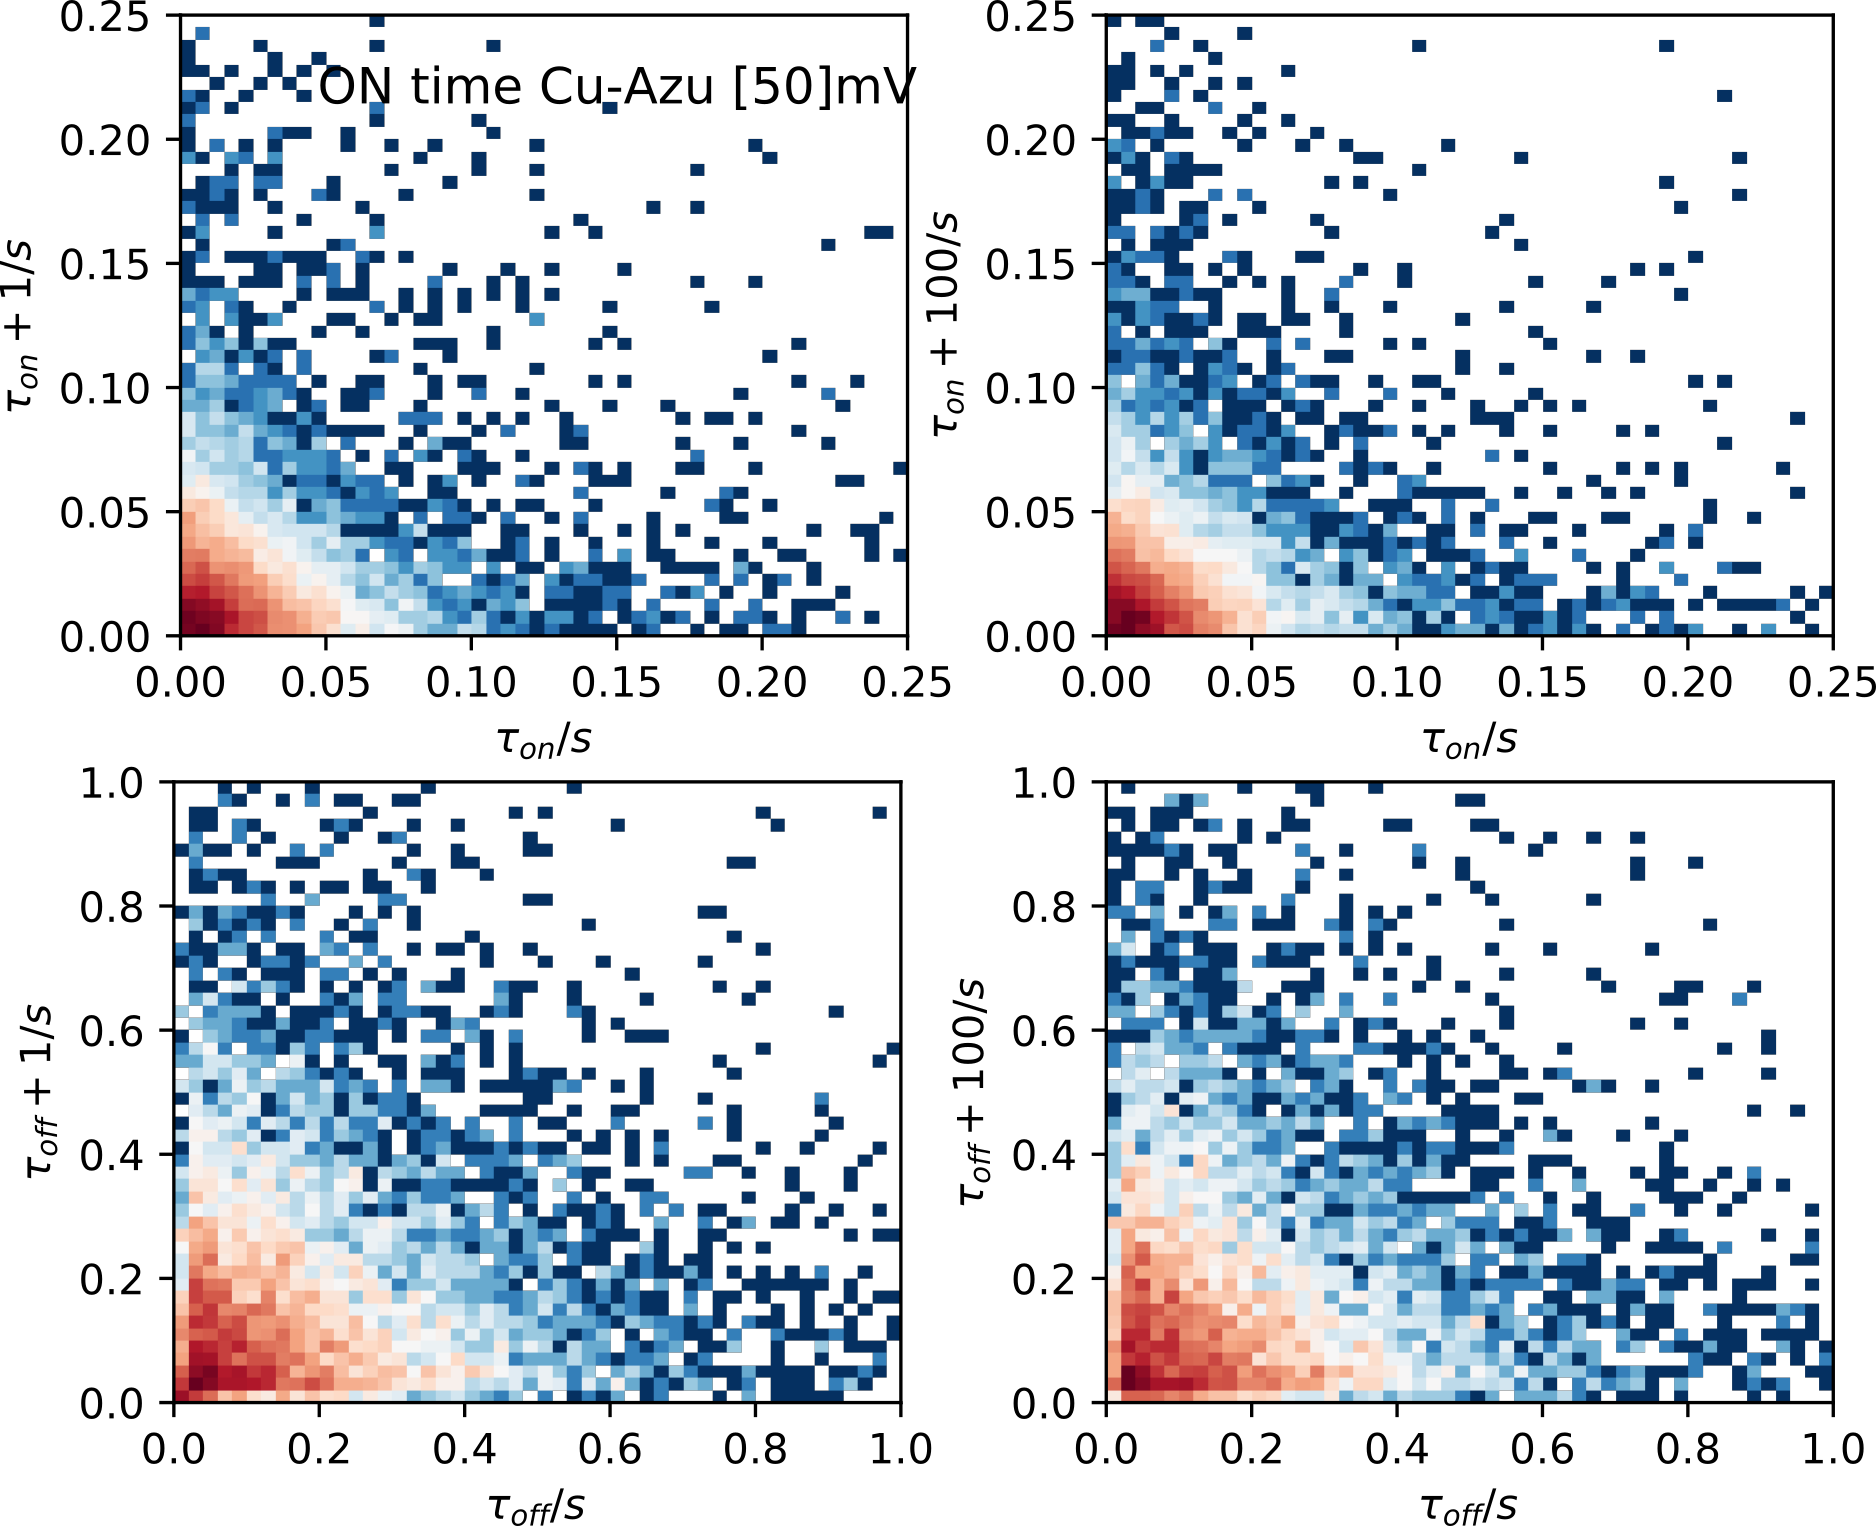
\includegraphics[width=\textwidth]{Figure_4_on_off_2D_100mV}
%   \makeatletter
%   \renewcommand{\fnum@figure}{\figurename~S\thefigure}
%   \makeatother
%   \caption{\textbf{2D histogram: Cu-Azurin.}Two-dimensional correlation plot of a single azurin at \SI{50}{\mV} of(a) adjacent waiting time for oxidation ($t_{n}~and~t_{n+1}$) (b) two waiting times at a large separation of 100 ($t_{n}~and~t_{n+100}$) (c) The difference two dimensional histogram of (a) and (b).}
%   \label{SIfig:onoff2D}
% \end{figure}